\documentclass[aspectratio=169,12pt]{beamer}
\usetheme{Madrid}
\usecolortheme{dolphin}
\usefonttheme{professionalfonts}
\setbeamertemplate{navigation symbols}{}
\setbeamertemplate{footline}{}

\usepackage[T1]{fontenc}
\usepackage[utf8]{inputenc}
\usepackage{graphicx}
\usepackage{amsmath,amssymb}
\usepackage{hyperref}
\usepackage{siunitx}
\usepackage{physics}

\begin{document}

\title[Chapter 3]{Chapter 3: Matrices, classical and quantum logic gates}
\author{JAMOTTE Maxime, SCHOONEN Cédric}
\institute{Digital Learning Hub}
\date{}

\begin{frame}
  \titlepage
\end{frame}

\begin{frame}{Chapter 3 objectives}
  \begin{enumerate}
    \item Matrices and their action on a vector\\~\\
    \item Operations on a qubit\\~\\
  \end{enumerate}
\end{frame}

\begin{frame}{Matrices and their action on a vector}
  {%
    \setbeamercolor{itemize/enumerate body}{fg=gray!60}
    \setbeamercolor{itemize item}{fg=gray!60}
    \setbeamercolor{alerted text}{fg=black}
    \begin{columns}[T]
      \begin{column}{0.55\textwidth}
        \begin{itemize}[<+-| alert@+>]
          \setlength{\itemsep}{0.6em}
          \item Matrix-vector multiplication
          \item Addition of matrices
          \item Multiplication of a matrix by a scalar
        \end{itemize}
        \bigskip
        \only<1>{\[M \vec{r} = 
          \begin{pmatrix} a & b \\ c & d \end{pmatrix}
          \begin{pmatrix} u \\ v \end{pmatrix} =
          \begin{pmatrix} au + bv \\ cu + dv \end{pmatrix}
        \]}
      \end{column}
      \begin{column}{0.4\textwidth}
        \centering
        \only<1>{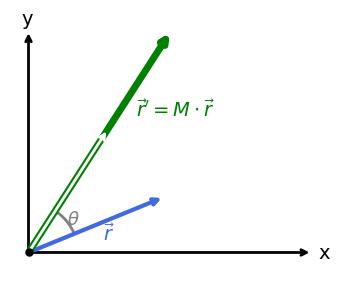
\includegraphics[width=\linewidth]{../figures/math/multiplication_Mv.png}}
        \only<2>{\fbox{\Large $M_1^{}+M_2^{}$}}
        \only<3>{\fbox{\Large $\lambda M$}}
      \end{column}
    \end{columns}
        \only<2>{\[M_1^{}+M_2^{} = 
          \begin{pmatrix} a & b\\ c & d \end{pmatrix} +
          \begin{pmatrix} e & f\\ g & h \end{pmatrix} =
          \begin{pmatrix} a+e & b+f\\ c+g & d+h \end{pmatrix}
        \]}
        \only<3>{\[ \lambda M = 
          \lambda \begin{pmatrix} a & b\\ c & d \end{pmatrix} =
          \begin{pmatrix} \lambda a & \lambda b\\ \lambda c & \lambda d \end{pmatrix}
        \]}
        
  }
\end{frame}



\begin{frame}{Matrix multiplication}

  \[ M_1 \times M_2 = \begin{pmatrix}
      {\color{red}a} & {\color{red}b} \\
      c & d
    \end{pmatrix}
    \begin{pmatrix}
      {\color{teal}u_1} & u_2 \\
      {\color{teal}v_1} & v_2
    \end{pmatrix}
    =
    \begin{pmatrix}
      {\color{red}a}{\color{teal}u_1} + {\color{red}b}{\color{teal}v_1} & au_2 + bv_2 \\
      cu_1 + dv_1 & cu_2 + dv_2
    \end{pmatrix}
  \]
\\~\\
\end{frame}

\begin{frame}{Matrix multiplication}

  \[ M_1 \times M_2 = \begin{pmatrix}
      {\color{red}a} & {\color{red}b} \\
      c & d
    \end{pmatrix}
    \begin{pmatrix}
      {\color{teal}u_1} & u_2 \\
      {\color{teal}v_1} & v_2
    \end{pmatrix}
    =
    \begin{pmatrix}
      {\color{red}a}{\color{teal}u_1} + {\color{red}b}{\color{teal}v_1} & au_2 + bv_2 \\
      cu_1 + dv_1 & cu_2 + dv_2
    \end{pmatrix}
  \]
\\~\\
    \textbf{Non-commutative} in general: $M_1 \times M_2 \neq M_2 \times M_1$.
  
  \bigskip
  \[
    \begin{pmatrix}
      0 & 1 \\
      1 & 0
    \end{pmatrix}
    \begin{pmatrix}
      1 & 0 \\
      0 & -1
    \end{pmatrix}
    =
    \begin{pmatrix}
      0 & -1 \\
      1 & 0
    \end{pmatrix}
      \]
  \bigskip
  \[
    \begin{pmatrix}
      1 & 0 \\
      0 & -1
    \end{pmatrix}
    \begin{pmatrix}
      0 & 1 \\
      1 & 0
    \end{pmatrix}
    =
    \begin{pmatrix}
      0 & 1 \\
      -1 & 0
    \end{pmatrix}
  \]
\end{frame}

\begin{frame}{Quantum operators on a qubit}
  \begin{itemize}[<+->]
    \setlength{\itemsep}{0.55em}
    \item The \textbf{vectors} representing \textbf{qubits} are transformed by \textbf{matrices}
     representing \textbf{quantum operators}.\\~\\
    \item Examples of single-qubit operators: Pauli X (inversion), Z (phase), Hadamard $H$ (creating superposition).\\~\\
  \end{itemize}
\end{frame}

\begin{frame}{$Z$ operation (phase)}
  Matrix notation:
  $$
    Z = \begin{pmatrix}1 & 0 \\ 0 & -1\end{pmatrix}
  $$\\~\\
  $$
    \begin{pmatrix}1 & 0 \\ 0 & -1\end{pmatrix}
    \begin{pmatrix}1\\0\end{pmatrix}=
    \begin{pmatrix}1\\0\end{pmatrix},
    \qquad
    \begin{pmatrix}1 & 0 \\ 0 & -1\end{pmatrix}
    \begin{pmatrix}0\\1\end{pmatrix}=
    \begin{pmatrix}0\\-1\end{pmatrix}
  $$
  ~\\~\\
  Operator notation: $$Z = \ket 0 \bra 0 - \ket 1 \bra 1$$\\~\\
  $$
    Z\ket 0 = \ket 0, \qquad
    Z\ket 1 = -\ket 1
  $$
  
\end{frame}


\begin{frame}{$X$ operation (quantum NOT)}
  Matrix notation:
  $$
    X = \begin{pmatrix}0 & 1 \\ 1 & 0\end{pmatrix}
  $$\\~\\
  $$
    \begin{pmatrix}0 & 1 \\ 1 & 0\end{pmatrix}
    \begin{pmatrix}1\\0\end{pmatrix}=
    \begin{pmatrix}0\\1\end{pmatrix},
    \qquad
    \begin{pmatrix}0 & 1 \\ 1 & 0\end{pmatrix}
    \begin{pmatrix}0\\1\end{pmatrix}=
    \begin{pmatrix}1\\0\end{pmatrix}
  $$
  ~\\~\\
  Operator notation: $$X = \ket 0 \bra 1 + \ket 1 \bra 0$$\\~\\
  $$
    X\ket 0 = \ket 1, \qquad
    X\ket 1 = \ket 0
  $$
  
\end{frame}



\begin{frame}{$H$ operation (Hadamard)}
  Matrix notation:
  $$
    H = \tfrac{1}{\sqrt{2}}\begin{pmatrix}1 & 1 \\ 1 & -1\end{pmatrix}
  $$\\~\\
  $$
    \tfrac{1}{\sqrt{2}}\begin{pmatrix}1 & 1 \\ 1 & -1\end{pmatrix}
    \begin{pmatrix}1\\0\end{pmatrix}=
    \tfrac{1}{\sqrt{2}}\begin{pmatrix}1\\1\end{pmatrix},
    \qquad
    \tfrac{1}{\sqrt{2}}\begin{pmatrix}1 & 1 \\ 1 & -1\end{pmatrix}
    \begin{pmatrix}0\\1\end{pmatrix}=
    \tfrac{1}{\sqrt{2}}\begin{pmatrix}1\\-1\end{pmatrix}
  $$
  ~\\~\\
  Operator notation: $$H = \tfrac{1}{\sqrt{2}} \ket 0 \bra 0 + \tfrac{1}{\sqrt{2}} \ket 0 \bra 1 + \tfrac{1}{\sqrt{2}} \ket 1 \bra 0 - \tfrac{1}{\sqrt{2}} \ket 1 \bra 1$$\\~\\
  $$
    H\ket 0 = \tfrac{1}{\sqrt{2}}(\ket 0+\ket 1), \qquad
    H\ket 1 = \tfrac{1}{\sqrt{2}}(\ket 0-\ket 1)
  $$
\end{frame}

\begin{frame}{End of chapter 3}
  \centering
  \vfill
  Let's move to hands-on practice with QISKIT!
  \vfill
\end{frame}

\end{document}
